\chapter{Selected Gamification Features for English Mind}

Based on the analysis of existing applications and their gamification features, we have identified several opportunities to enhance the English Mind application. Our selection process focused on features that meet three key criteria:

\begin{enumerate}
    \item \textbf{High Impact Potential:} Features that have demonstrated effectiveness in other applications and show strong potential for improving user engagement and learning outcomes.
    
    \item \textbf{Alignment with Core Concepts:} Features that complement and enhance English Mind's fundamental learning principles of frequency-based vocabulary acquisition and spaced repetition.
    
    \item \textbf{Implementation Feasibility:} Solutions that can be realistically implemented within the existing application architecture and technical constraints.
\end{enumerate}

Rather than attempting to implement every possible gamification feature, we have prioritized a focused set of enhancements that we believe will provide the most significant benefits to users. These proposed features have been organized into two main categories:

\begin{itemize}
    \item \textbf{Enhanced Practice Experience:} Improvements to the core flashcard practice system to make it more engaging and effective (see Section \ref{sec:em-gamification-practice-experience}).
    
    \item \textbf{Consistent Practice Motivation:} Features designed to encourage regular app usage and maintain long-term user engagement (see Section \ref{sec:em-gamification-practice-motivation}).
\end{itemize}

For each proposed feature, we have developed detailed high-fidelity prototypes and implementation considerations. These designs demonstrate how each gamification element will be integrated into the existing application while maintaining its core educational value.

\section{Enhanced Practice Experience}
\label{sec:em-gamification-practice-experience}
The core flashcard practice experience is fundamental to English Mind's learning methodology. While the current implementation is functional, our analysis revealed several opportunities to make it more engaging and effective through gamification. This section presents three key enhancements to the practice experience, each designed to increase user engagement while maintaining the app's educational integrity.

\subsection{Diversified Flashcard Types}

The current English Mind flashcard system uses a single format where users view an English word and recall its meaning. While effective, our analysis of similar applications revealed that incorporating multiple flashcard types can enhance engagement and address different aspects of vocabulary acquisition. We propose expanding the system to include five distinct flashcard types, each targeting specific learning objectives (see Figure \ref{fig:em-prototype-flashcard-types}).

\begin{itemize}
    \item \textbf{Basic Meaning Recognition (Existing)}

    The current format where users see an English word and recall its meaning will be maintained as the foundation of the practice system. This format effectively tests basic word recognition and meaning recall (see Section \ref{sec:em-active-recall-flashcards}).

    \item \textbf{Word Matching (Two Variants)}
    
    Following the successful implementation in applications like Duolingo and WordUp, we propose two matching exercise variants:
    
    \begin{itemize}
        \item \textbf{Word-Translation Matching:} Users match English words with their corresponding translations, presented in sets of five pairs.
        
        \item \textbf{Word-Definition Matching:} Similar to the translation variant, but users match English words with their definitions, reinforcing deeper understanding of word meanings.
    \end{itemize}

    \item \textbf{Word Spelling}
    
    This exercise type presents users with a word's definition and a contextual sentence containing a blank space. Users must correctly spell the target word to complete the sentence. To assist learning, an audio pronunciation button is available. The system evaluates spelling accuracy and provides immediate feedback.
    \newpage

    \item \textbf{Word Pronunciation}

    Users are shown an English word and prompted to pronounce it correctly. The flashcard displays both the word and its IPA (International Phonetic Alphabet) transcription. The system evaluates pronunciation accuracy using speech recognition technology, providing binary feedback (correct/incorrect). Understanding that not all practice environments are suitable for speaking exercises, users can opt to skip these cards when needed.

\end{itemize}

\begin{figure}[!h]
    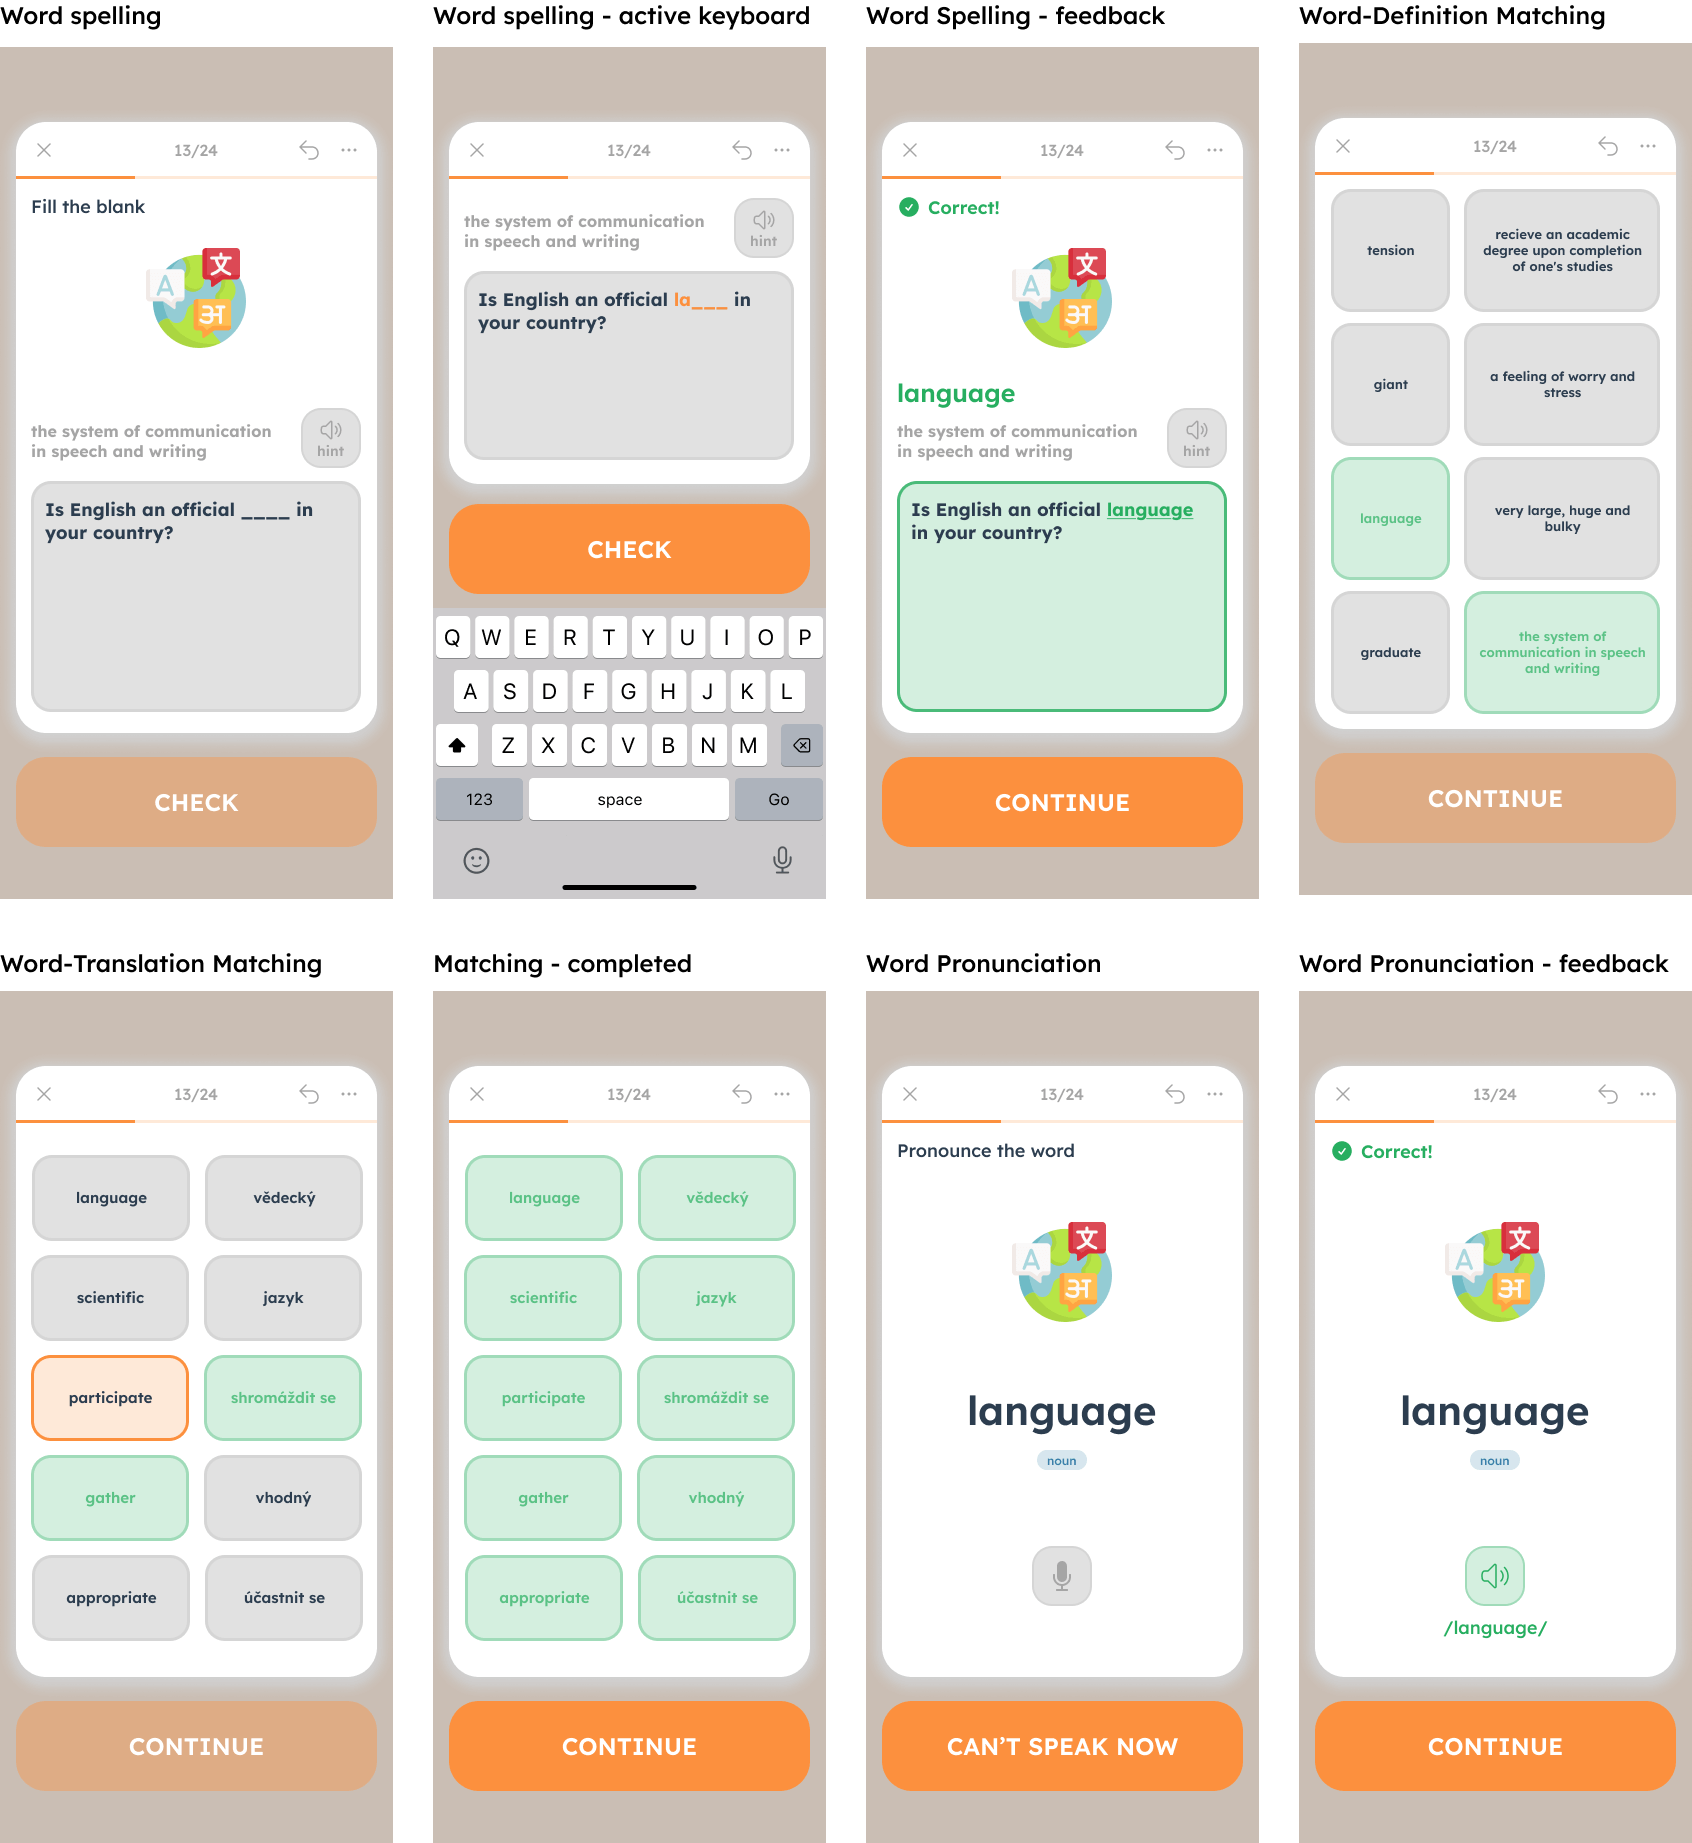
\includegraphics[width=1\textwidth]{src/figures/em-prototype-flashcards.png}
    \caption{English Mind - Prototype: Flashcard Types}
    \label{fig:em-prototype-flashcard-types}
\end{figure}

\subsubsection{Implementation Considerations}

The integration of new flashcard types requires careful consideration of both the spaced repetition system and the distribution of different card types during practice sessions.

To maintain the integrity of the existing spaced repetition system, only the basic meaning recognition flashcards will carry spaced repetition metadata and influence the scheduling of words. The additional flashcard types will serve as supplementary practice exercises without affecting the core SRS algorithm. This approach ensures the proven effectiveness of the current SRS remains unchanged, while additional practice types enhance learning without disrupting the established review schedule. Furthermore, this design allows user progress tracking to remain clear and consistent throughout the learning process.

The distribution of flashcard types within a practice session follows a structured approach that ensures varied practice while maintaining focus on core vocabulary acquisition through the primary flashcard type:

\begin{itemize}
    \item \textbf{Primary Flashcards:} Basic meaning recognition flashcards appear first in the daily queue, maintaining their role as the foundation of the spaced repetition learning system.
    
    \item \textbf{Supplementary Flashcards:} After completing the primary flashcards, users encounter the following types in randomized order:
    \begin{itemize}
        \item \textbf{Matching Flashcards:} Appear once for every five words in practice, grouping words into logical sets
        \item \textbf{Spelling Flashcards:} Randomly distributed throughout the supplementary practice
        \item \textbf{Pronunciation Flashcards:} Limited to newly introduced words and appear less frequently than other types
    \end{itemize}
\end{itemize}

\subsubsection{Expected Impact}

The diversification of flashcard types is expected to yield several benefits:

\begin{itemize}
    \item \textbf{Enhanced Engagement:} Variety in flashcard types reduces monotony and maintains user interest throughout longer practice sessions.
    
    \item \textbf{Comprehensive Learning:} Different flashcard types target various aspects of vocabulary acquisition, leading to more robust word knowledge.
    
    \item \textbf{Improved Retention:} Encountering words through different exercise types (recognition, matching, spelling, and pronunciation) creates multiple memory pathways, leading to stronger and longer-lasting vocabulary retention.
    
\end{itemize}

\subsection{Individual Word Progress Tracking}
% Visual progress indicator for each word
% Integration with existing SRS system
% Wireframes showing progress visualization
% Expected impact on user motivation

\subsection{Post-Practice Review}
% End-of-session summary screen
% Practice statistics
% Wireframes for review screen
% Expected impact on user engagement

\section{Consistent Practice Motivation}
\label{sec:em-gamification-practice-motivation}
% This section focuses on features that encourage regular use

\subsection{Daily Goals and Streak System}
% Enhanced visualization of daily word goals
% Progress tracking throughout the day
% Wireframes for goal visualization
% Expected impact on daily engagement
% Daily streak tracking mechanism
% Streak protection features
% Notification strategy
% Wireframes for streak visualization
% Expected impact on long-term retention